e^{2}\,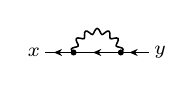
\begin{tikzpicture}[x=0.600cm, y=0.600cm, line width=0.550pt, baseline={([yshift=-0.6ex]0,0)}]
  \draw (0.500,0.000) -- (-0.500,0.000);
  \fill (-0.089,0.000) -- (0.089,-0.076) -- (0.031,0.000) -- (0.089,0.076) -- cycle;
  \draw plot[smooth, tension=0.7] coordinates {(-0.500,0.000) (-0.537,0.035) (-0.548,0.069) (-0.524,0.095) (-0.476,0.110) (-0.427,0.121) (-0.401,0.138) (-0.405,0.168) (-0.427,0.213) (-0.445,0.260) (-0.441,0.296) (-0.407,0.308) (-0.357,0.301) (-0.308,0.290) (-0.278,0.293) (-0.268,0.322) (-0.269,0.372) (-0.265,0.423) (-0.245,0.453) (-0.209,0.450) (-0.167,0.422) (-0.128,0.390) (-0.099,0.380) (-0.078,0.402) (-0.057,0.447) (-0.031,0.491) (0.000,0.509) (0.031,0.491) (0.057,0.447) (0.078,0.402) (0.099,0.380) (0.128,0.390) (0.167,0.422) (0.209,0.450) (0.245,0.453) (0.265,0.423) (0.269,0.372) (0.268,0.322) (0.278,0.293) (0.308,0.290) (0.357,0.301) (0.407,0.308) (0.441,0.296) (0.445,0.260) (0.427,0.213) (0.405,0.168) (0.401,0.138) (0.427,0.121) (0.476,0.110) (0.524,0.095) (0.548,0.069) (0.537,0.035) (0.500,0.000)};
  \draw (-0.500,0.000) -- (-1.100,0.000);
  \fill (-0.919,0.000) -- (-0.741,-0.076) -- (-0.799,0.000) -- (-0.741,0.076) -- cycle;
  \draw (0.500,0.000) -- (1.100,0.000);
  \fill (0.681,0.000) -- (0.859,-0.076) -- (0.801,0.000) -- (0.859,0.076) -- cycle;
  \fill (-0.500,0.000) circle (0.064);
  \fill (0.500,0.000) circle (0.064);
  \node[font=\scriptsize, inner sep=0pt, anchor=0] at (-1.190,0.000) {$x$};
  \node[font=\scriptsize, inner sep=0pt, anchor=180] at (1.190,0.000) {$y$};
\end{tikzpicture}